\documentclass[12pt,twoside]{article}
\usepackage[a4paper,width=150mm,top=30mm,bottom=30mm,bindingoffset=10mm]{geometry}
\linespread{1}
\usepackage[utf8]{inputenc} %Standard diacritics in Romance languages (accents, umlauts)
\usepackage{newtxtext} %Uses Times New Roman font
\usepackage[nointegrals]{wasysym}
\usepackage{ragged2e}
\usepackage{diagbox}
\usepackage[labelfont=bf,labelsep=period,font=small,justification=RaggedRight,format=plain,margin=0pt,singlelinecheck=false]{caption}
\usepackage{graphicx}
\graphicspath{ {./images/} }
\usepackage[style=authoryear-icomp,natbib=true,sortcites=true,maxbibnames=99]{biblatex}% natbib=true so we can use natbib commands with biblatex
% Also: authoryear-icomp is used so that when you cite the same author with different years, you get "according to Herberger (2002, 2004)" rather than "according to Herberger (2002), Herberger (2004)"
% maxbibnames=99 lists all full names in the bibliography rather than using "et al", as specified in Isogloss's formatting guidelines
\addbibresource{isogloss.bib}

\usepackage{xpatch}

%\usepackage[tiny,bf]{titlesec}
%\titleformat{\subsection}{}{\thesubsection}{1em}{\itshape}
%\titleformat{\subsubsection}{}{\thesubsubsection}{1em}{\itshape}
\usepackage[tiny]{titlesec}
\newcommand{\periodafter}[1]{#1.}
\titleformat{\subsection}{\itshape}{\thesubsection\periodafter}{0.3em}{\itshape}
\titleformat{\subsubsection}{\itshape}{\thesubsubsection\periodafter}{0.3em}{\itshape}
\titlelabel{\thetitle.\quad}
\setlength\parindent{1.25cm}
\titlespacing*{\subsection}{0pt}{1em}{0pt}
\titlespacing*{\subsubsection}{0pt}{1em}{0pt}

\usepackage{fancyhdr}
\pagestyle{fancy}
\fancyhead{}
\fancyhead[LE]{\thepage \hspace{3mm} \small Isogloss YEAR, ISSUE/NR}
\fancyhead[RE]{\small Daniel Stelzer}
\fancyhead[LO]{\small Title of paper [leave `Title of paper' unchanged]}
\fancyhead[RO]{\small Isogloss YEAR, 1/2 \normalsize \thepage}
\fancyfoot{}
%\setcounter{page}{23} %This sets the initial page at a number other than 1 (in this case 23).

\fancypagestyle{first}{
	\fancyhead{}
	\fancyhead[L]{\small ISSN 2835-4138 (digital)\\https://doi.org/10.5565/rev/isogloss.\\{}}
	\fancyhead[R]{\small Isogloss YEAR, ISSUE/NR\\PAGES\\{}}
	\fancyfoot{}}

\newcommand{\pref}[1]{(\ref{#1})} % If you use \ref{xx}, the reference in the text appears without parentheses: "as we see in 1, ..." instead of "as we see in (1)...". So we create a new command: instead of \ref, call \pref (Parentheses REFerence) which specifies that any cross references to xx appear in parentheses.

% The following syntax, in tandem with xpatch package, removes the brackets in the references list. It also removes the dot after the line.
% See https://tex.stackexchange.com/a/428193/169121
\xpatchbibmacro{date+extradate}{%
	\printtext[parens]%
}{%
\setunit{\addperiod\space}%
\printtext%
}{}{}

% Change page number formatting to "Details: Pages" instead of "Details, pp. Pages" in both cites and bibliography
\renewcommand{\bibpagespunct}{\addcolon\space}
\renewcommand{\postnotedelim}{\addcolon\space}
\DeclareFieldFormat{pages}{#1}
\DeclareFieldFormat{postnote}{#1}

\usepackage{tipa} %for IPA
\usepackage{phonrule} %for phonological rules
\usepackage[nocenter]{qtree} %for trees
\usepackage{gb4e} %for examples and glossing
\noautomath % Don't break everything with underscores please!

\usepackage[normalem]{ulem} %STRIKETHROUGH TEXT

\usepackage{authblk,etoolbox}
\renewcommand\Authfont{\Large}
\renewcommand\Affilfont{\normalsize}

\usepackage{amsmath}
\usepackage{citeposs}
\usepackage{tablefootnote}
\usepackage{xcolor}
\usepackage{colortbl}
\newcommand{\ipa}[1]{/\textipa{#1}/}
\newcommand{\ipab}[1]{[\textipa{#1}]}
\newcommand{\yields}{\textrightarrow}
\DeclareGraphicsExtensions{.pdf,.png}

\usepackage{hyperref}
\newcommand*{\tocref}[1]{\hyperref[{#1}]{\ref*{#1}.~\nameref*{#1}}}
% https://tex.stackexchange.com/q/121865/169121
\hypersetup{ % TODO is this okay?
	colorlinks,
	linkcolor={red!75!black},
	citecolor={blue!50!black},
	urlcolor={blue!80!black}
}

\makeatletter
% patch \maketitle so that it doesn't center
\patchcmd{\@maketitle}{center}{flushleft}{}{}
\patchcmd{\@maketitle}{center}{flushleft}{}{}
% patch \maketitle so that the font size for the title is normal
\patchcmd{\@maketitle}{\LARGE}{\normalsize}{}{}

\def\maketitle{{%
		\renewenvironment{tabular}[2][]
		{\begin{flushleft}}
			{\end{flushleft}}
		\AB@maketitle}}
\makeatother

\title{{\Huge{}How fast did Cicero speak?}\\{\Large{}The speech rate of Classical Latin versus its Romance descendants}}
\author{Daniel Stelzer}
\affil{University of Illinois at Urbana-Champaign\\stelzer3@illinois.edu}
\setlength{\affilsep}{1pt}
\date{}

%IF THERE ARE TWO AUTHORS:
%\title{\Huge{Patterns of syntactic microvariation: the case of European Portuguese}}
%\author{Noam Chomsky} \affil{Massachusetts Institute of Technology\\noam.chomsky@mit.edu} 
%\author{Howard Lasnik} \affil{University of Maryland\\howard.lasnik@umd.edu}
%\setlength{\affilsep}{1pt}
%\date{}

\begin{document}


\maketitle

\thispagestyle{first}

\vspace{0.5cm}
\noindent \includegraphics[height=1cm]{ccby.png}

\hfill Received: XX-XX-XX

\hfill Accepted: XX-XX-XX

\hfill Published: XX-XX-XX

\vspace{1cm}

\noindent \textbf{How to cite} [Leave blank]

\vspace{1.5cm}

\noindent \textbf{Abstract}
\begin{center}
 	\line(1,0){430}
\end{center}
\vspace{-0,3cm}
\noindent While languages convey significantly different amounts of both information per syllable and syllables per second, recent research suggests that the product of these values---information conveyed per second---is much less variable. Using new methods of extrapolation and resampling, we were able to estimate the information conveyed per syllable in a written Classical Latin corpus. We were then able to use this cross-linguistic consistency to estimate the natural speech rate of Classical Latin, a language that hasn't been natively spoken for thousands of years. Our analysis suggests that it was spoken at a rate significantly slower than modern Romance languages, fairly similar to modern English; a high-level consideration of historical sound changes in Romance supports this conclusion, lending additional credence to our results.

\vspace{5mm}

\noindent \textbf{Keywords:} Information density; speech rate; Latin; information theory; resampling.

\vspace{4mm}
\begin{center}
	\line(1,0){430}
\end{center}

%\begin{center}
	%\textbf{Table of Contents}
%\end{center}

%\begin{large}
%\begin{center}
	%\begin{tabular}{l l}
		%\tocref{sec:bg} & \tocref{sec:disc} \\
		%\tocref{sec:meth} & \tocref{sec:concl} \\
		%\tocref{sec:res} & \hyperref[sec:refs]{References} \\
	%\end{tabular}
%\end{center}
%\end{large}

\section{Background}
\label{sec:bg}

The idea that all languages are equally expressive---that, despite all the variation in phonology, syntax, and other aspects, every language is equally suited to communication and equally complex or sophisticated in its grammar---is ubiquitous in modern linguistics. \citet{joseph} attribute the earliest expression of this concept to Humboldt in the 1820s, who claimed that ``all [languages] contain all that is rigorously needed not only for the correctness, but the perfection of expression''\footnote{Quoted in \cite[8]{rémusat}; translation from \cite[344]{joseph}.}. By the end of the 19th century, this idea had gained support from the study of language evolution: \citet[227]{passy} suggested that language change is an eternal struggle between the tendencies ``to get rid of what is superfluous'' and ``to highlight what is necessary''\footnote{Translation from \cite[352]{joseph}.}, preventing any overall increase or decrease of complexity.

Despite significant pushback, especially from those who bristled at the idea of equating European languages with those of Africa and the Americas, this idea slowly gained traction among the linguistic community; by 1955 it had made its way into the \emph{Encyclopædia Britannica} article on ``Language'', now with a specific mention of ``complexity'': ``All languages of today are equally complex and equally adequate to express all the facets of the speakers' culture, and all can be expanded and modified as needed'' \citep[698]{trager}. While the idea of ``primitive'' versus ``sophisticated'' languages persists in pop culture, this hypothesis of equal complexity is now put forth as a basic axiom in introductory textbooks: \citet[8]{akmajian}, for example, state plainly that ``all known languages are at a similar level of complexity'', and \citet[8]{ogrady} assert that ``linguists don't even try to rate languages as [\,\ldots] simple or complex''\footnote{Outside of introductory textbooks, some linguists are more skeptical. \citet[2]{shosted} refers to it as ``a claim that has been, until fairly recently, more a matter of dogma than of science'', and \citet[216]{maddieson} suggests that ``[s]uch a view seems to be based on the humanistic principle that all languages are to be held in equal esteem and are equally capable of serving the communicative demands placed on them. In rejecting the notion of `primitive' languages linguists seem to infer that a principle of equal complexity must apply.'' On the flipside, other linguists support the claim for purely theoretical reasons: \citet[165-166]{chomsky} suggests that all languages ``ought to'' have the same overall budget for markedness, no matter how they spend it. \citet[540]{pellegrino} suggest simply that ``the assumption of an `equal overall complexity' is ill-defined''. For more discussion, see \cite{joseph}.}.

% Maddieson 216: "Such a view seems to be based on the humanistic principle that all languages are to be held in equal esteem and are equally capable of serving the communicative demands placed on them. In rejecting the notion of `primitive' languages linguists seem to infer that a principle of equal complexity must apply."

However, what exactly this universal ``expressiveness'' (or ``complexity'' or ``sophistication'') \emph{means} is far from obvious. Many typological studies, such as \citet{maddieson} and \citet{shosted}, have tried to quantify the complexity of different aspects of grammar, looking for correlations between them (e.g.\ complicated phonology correlating with simpler morphology)---but results have generally been inconclusive.

In the 1950s, this trend of research was given a new suite of tools from the burgeoning discipline of information theory. \citet{shannon} introduced new mathematical models of information transmission based on concepts like entropy, noise, and channel capacity, and mathematically-inclined linguists soon started applying these models to spoken language. \citet[674,676]{karlgren}, for example, suggested that ``seemingly careless pronunciation'' was actually ``an efficient coding to fit the channel'' of vocal transmission, and in particular that ``there is an equilibrium between [Shannon's] information value on the one hand and duration and similar qualities of the realization on the other''.

% \textbf{THE FOLLOWING PARAGRAPHS ARE NEW}

While \citeauthor{karlgren} failed to find significant correlations between the lengths of words and the ``carelessness'' of speech \citep{karlgren}, the appeal of channel-focused models persisted. \citet{lieberman} attempted to measure the redundancy of various elements of a sentence, and found that the less redundant (i.e. more informative) elements were pronounced louder and longer. The word ``nine'' in the phrase ``a stitch in time saves nine'', for example, is extremely redundant: after hearing the five previous words, you know exactly what's coming next. The word ``nine'' in ``that will be nine dollars'', on the other hand, will significantly impact a listener's understanding of the sentence---and thus, it is pronounced more distinctly. Further experiments in the following decades supported \citeauthor{lieberman}'s results\footnote{See \cite[32]{aylett} for further references on these studies.\citereset}, and \citet{aylett} expanded these into a general principle, which they termed the ``Smooth Signal Redundancy Hypothesis'' \citep[34]{aylett}.

According to this hypothesis, speakers aim to have a similar level of redundancy across different parts of an utterance. If a phrase has a low level of linguistic redundancy (i.e. it's difficult to predict from context), it will show a higher level of acoustic redundancy (i.e. it will be pronounced clearly and carefully), and vice versa. The experimental evidence was promising, and \citet{jaeger} extended it into what he termed the ``Uniform Information Density Hypothesis''. Speakers, \citeauthor{jaeger} predicted, should structure their syntax to convey a consistent rate of information over time: sculpting their language to fit what \citet{shannon} would call the ``channel capacity'' \citep[3]{jaeger}.

Preliminary experiments with both production and comprehension have supported this hypothesis, suggesting that \citeauthor{shannon}'s information theory might be, in fact, a good model of human language \parencites[29]{jaeger}[970-971]{meister}. If so, this could offer a new way of measuring languages' complexity, using information-theoretic methods. As \citet[539]{pellegrino} put it, ``[l]anguage is actually a communicative system whose primary function is to transmit information. The unity of all languages is probably to be found in this function, regardless of the different linguistic strategies on which they rely.''

Since then, many authors have continued to examine language ``complexity'' through this lens \citep{pellegrino,oh,coupé}. In particular, while acquiring acoustic data is still fairly time-consuming, access to written corpora has grown dramatically in recent years. Corpora with hundreds of millions of tokens have become common, and web-based English corpora easily reach the billions. \citet{oh} takes advantage of this data, analyzing the information density in written corpora from 18 languages and proposing a number of different metrics to investigate the Uniform Information Density Hypothesis in greater depth.

Some linguists, conversely, have questioned whether information-theoretic entropy is an appropriate metric for measuring the information content of natural language. After all, \citet[8]{shannon} themselves specifically note that ``[t]he word \emph{information}, in this theory, is used in a special sense that must not be confused with its ordinary usage. In particular, \emph{information} must not be confused with meaning.'' Information theory defines ``information'' as a specific mathematical quantity, based on signals sent through a channel. But is that necessarily the same as the meaning that humans try to convey through language?

\citet{pellegrino} searched for a different cross-linguistic measure of semantic density, in order to analyze how \emph{meaning} (rather than Shannon's \emph{information}) is encoded for verbal communication. The metric they came up with was based on the ratio of syllables in parallel corpora---in other words, the number of syllables that experienced translators use to convey the meaning of a particular text in a language, compared to the number of syllables needed to convey that same text in a control language.

% \textbf{NOW BACK TO OLD STUFF}

Using this measure, they found a striking negative correlation between the density of semantic meaning per syllable (``meaning density''\footnote{``Meaning density'' is my own terminology, to avoid ambiguity; \citet{pellegrino} and \citet{oh} call it ``information density'' (ID) or occasionally ``semantic information density'', while \citet{coupé} call it ``syntagmatic density of information ratio'' (SDIR).}) and the number of syllables spoken per second (``speech rate'') in different languages. In the end, they rejected the hypothesis that the amount of meaning conveyed per second was uniform between languages---with a note that ``[t]he very small size of the sample (N=7 languages) strongly limits the reliability of the results'' \citep[550]{pellegrino}. They were also limited by relatively small corpora---20 texts of 5 sentences each---and were not able to control for the effects of individual translators' style\footnote{It should be noted, though, that their corpora were significantly larger than those used in previous studies. For more details, see \citereset\cite[545]{pellegrino}.}.

These results by \citet{oh} and \citet{pellegrino} were brought together by \citet{coupé}, who first showed that one of \citeauthor{oh}'s corpus-based information density metrics was a good (and easier-to-calculate) proxy for \citeauthor{pellegrino}'s meaning density\footnote{However, the sample size in \citeauthor{pellegrino}'s study was fairly small. The relationship between ``information'' and ``meaning'' certainly merits further study, especially now that parallel corpora have become more available.}, then applied it to a wide variety of languages using larger written corpora. They found that the amount of information conveyed per second (``information rate'') was extremely consistent across the languages surveyed: while not perfectly constant (speech rate varies significantly by speaker and circumstance, for example), this average information rate varies much less by language than speech rate or information density, and seems to generally stay within a particular narrow band. They suggest that this ``optimal range'' is a result of ``universal communicative pressures characterizing the human-specific communication niche'' \citep[6]{coupé}. In other words, information rate is a property of how humans use language to communicate, on a larger scale than any individual language: ``social and neurocognitive pressures [\,\ldots] define an optimal range for [information rate], around which the complex adaptive system (consisting of each language and its speakers) hovers'' \citep[6]{coupé}.

The present study is a new application of \citeauthor{coupé}'s results. Speech rate is normally calculated through recordings of native speakers, which is impossible for a dead language like Classical Latin\footnote{\citeauthor{oh} also investigated the speech rate of bilinguals in \cite{ohbilingual}. The results were not conclusive but suggest that the speech rate of L2 speakers can vary significantly from L1 speakers, meaning classicists who become fluent later in life cannot reliably tell us the speech rate of native speakers in ancient Rome.}. However, \citeauthor{oh}'s methods of calculating information density are based on \emph{written} corpora, which do exist for a number of extinct languages. If we assume the optimal information rate is constant across time and culture, can we calculate the information density from a corpus, and thereby ``reverse engineer'' the speech rate?

% Coupé 6: "social and neurocognitive pressures [\ldots] define an optimal range for IR, around which the complex adaptive system (consisting of each language and its speakers) hovers."

% Pellegrino 539: "Language is actually a communicative system whose primary function is to transmit information. The unity of all languages is probably to be found in this function, regardless of the different linguistic strategies on which they rely."

% Shannon and Weaver 8: "The word \emph{information}, in this theory, is used in a special sense that must not be confused with its ordinary usage. In particular, \emph{information} must not be confused with meaning."

\section{Methods}
\label{sec:meth}

\subsection{Entropy}
\label{subsec:entropy}

The concept of entropy, as used in this study, was first proposed by \citet{shannon} as a way of quantifying information content. Shannon's model of communication involves an ``information source'' emitting a series of discrete ``signals'', one after another; in our model, the information source is a speaker (or writer) of a language, and the signals are syllables.

The ``entropy'' of an information source then measures how much information, on average, each new signal conveys---or, equivalently, how much we \emph{don't know} about a signal before we see it\footnote{Hence the name ``entropy''. In statistical mechanics, entropy is a measure of uncertainty.}. The original formulation from \citet[50]{shannon} is now known specifically as the \emph{Shannon entropy}:

\begin{equation}
\label{eqn:shannon}
H = - \sum_x P(x) \log P(x)
\end{equation}

Where \(x\) is a type of signal and \(P(x)\) is the probability of that signal. Intuitively, this means that information sources with more balanced probabilities will have higher entropy (if some types of signals are much more common than others, it's easier to guess what's coming next), and information sources with more types of signals will have higher entropy (if there are more possibilities, it's harder to guess what's coming next).

For our purposes, though, \citet{oh} suggests a slightly different model. In actual speech, signals don't exist in a vacuum devoid of context---mathematically, they're not independent. Consider, for example, English letters as signals. Without any context, the entropy is fairly high, since there are quite a lot of common letters to choose from. But right after a \textsc{q}, the next letter is almost certain to be a \textsc{u}; we can be very confident what letter is coming next, giving the source an extremely low entropy in this situation. To model this, \citet[52]{shannon} also propose what is now called the \emph{conditional entropy}:

\begin{equation}
H_c = - \sum_{x,c} P(c,x) \log \frac{P(c,x)}{P(c)}
\end{equation}

Where \(c\) is some representation of the context. In \citeauthor{oh}'s model, specifically, the signals are syllables of a language, and the context is the preceding syllable within the same word (making it a syllable bigram model)\footnote{See \cite[41]{oh} for a worked example, using a toy language for demonstration; see \cite[545]{pellegrino} for a discussion of using syllables versus phonemes as units.}. This is the metric used by \citet{coupé}, who term it ID (Information Density)\footnote{As mentioned in section~\ref{sec:bg}, comparison with \posscite{pellegrino} meaning density suggests this is a good measure of semantic content, though this relationship deserves further study.}:

\begin{equation}
\label{eq:id}
ID = - \sum_{\substack{\textrm{syllable},\\\textrm{context}}} P(\textrm{context, syllable}) \log \frac{P(\textrm{context, syllable})}{P(\textrm{context})}
\end{equation}

Our implementation follows \posscite[39]{oh} method exactly, using frequencies in a large corpus to approximate signal probabilities. Notably, we only consider context within a single word, not between words. This limitation was imposed by the corpora \citeauthor{oh} used, many of which only provide individual word frequencies; we continue with it both to ensure our results can be compared directly against \posscite{coupé}, who hewed similarly closely to \citeauthor{oh}'s methods, and to avoid the question of which boundaries (phrase, clause, sentence, paragraph, book) context should be able to cross\footnote{See, however, the comments in section~\ref{sec:concl}.}.

\subsection{Representation}
\label{subsec:repr}

The input to the bigram model discussed in section \ref{subsec:entropy} is a broad\footnote{Though since the entropy is calculated on the syllable level rather than the phoneme level, and context is taken into account, the narrowness of the transcription is less important than for Shannon entropy.} phonemic representation, with syllable boundaries marked. Since our corpus consists of plain text, we need a way of converting it to this phonemic representation. We accomplish this in three steps: augmenting the original orthography with additional data, converting the augmented orthography to a phonemic representation, and breaking this representation into syllables.

Fortunately, Classical Latin orthography is very close to phonemic. The Latin alphabet was still being modified during the Classical era, and deliberately-archaic spellings were rare\footnote{Archaisms were rare, but not unheard of. The archaic forms \emph{quom} `when' and \emph{com} `with' both became \emph{cum} in Classical times due to a sound change, for example, leading some authors to use archaizing spellings to distinguish them. While the homonymy muddies the waters somewhat, the numbers here are illuminating: \emph{quom} is attested 780 times in our corpus, \emph{com} 3, and \emph{cum} 55,738.}. This means that, for the most part, Classical orthography is thought to accurately represent the way the language was spoken at that time \citep[9]{allen}. However, some phonemic distinctions remain unrepresented, such as vowel quantity and vowels versus semivowels:

% quom 780
% com 3
% cum 55,738

\begin{exe}
\ex \textsc{alivm} \ipa{a.li.um} `another'
\ex \textsc{alivm} \ipa{a:.li.um} `garlic'
\ex \textsc{volvit} \ipa{wo.lu.it} `she wanted'
\ex \textsc{volvit} \ipa{wol.wit} `it rolls'
\end{exe}

To account for this, we first convert the corpus to an ``augmented'' or ``annotated'' orthography, which distinguishes \emph{a} from \emph{\=a}, \emph{u} from \emph{v}, and so on. This orthography is often used in introductory textbooks and is given here in \emph{italics}, as opposed to \textsc{smallcaps} for the original orthography found in the corpus; by design, it unambiguously represents all native phonemic differences.

Manually annotating a text in this way is generally straightforward---metered poetry and etymology reveal the quantity of most vowels, for example---but is extremely time-consuming. As a result, most documents in the corpus have never been manually annotated. For our analysis, we rely on an automatic annotation system developed by \citet{winge}\footnote{The system is available at \url{https://github.com/Alatius/latin-macronizer}, with an online demonstration at \url{https://alatius.com/macronizer/}.}, the heart of which is a customized version of \posscite{crane} Morpheus database. \citet[27]{winge} reports an accuracy exceeding 98\% on classical texts, which is sufficient for our purposes.

% Note: the version of CLTK used is specifically version 0.1.122, available at
% https://github.com/cltk/cltk/tree/22fabfd4e26f677ecce30871af78561edefcaef6
% It has not been tested with any later versions! In particular, the following major release completely overhauled the API, likely breaking everything
% This particular version is also not available on PyPI; it needs to be downloaded from Github instead

The conversion from augmented orthography to phonemic representation is very regular, and mostly consists of handling quirks of the writing system. The augmented orthography is unambiguous, but still sometimes uses one letter for a sequence of multiple phonemes (\emph{x} \ipa{ks}) or vice versa (\emph{qu} \ipa{k\super{w}})\footnote{See \texttt{data/latin/process.py} for the full details.}. Following \citet{allen}, we generally assume that a distinction in writing indicates a distinction in pronunciation---for example, the fact that the Greek letters \textsc{y} and \textsc{z} were borrowed during this period to transcribe loans implies that educated speakers really did pronounce them differently from \textsc{i} and \textsc{s}, and they should be treated as distinct phonemes. Similarly, spelling variations in transparent compounds like \emph{ad-sum}\textasciitilde\emph{as-sum} `I am here' are taken to indicate actual variation between analogical and expected pronunciations\footnote{Compare \citet[22]{allen}: ``It is in fact uncertain to what extent in educated speech the analogical spellings may also have been reflected in pronunciation.'' Our choice to take these spellings at face value was in part motivated by ease of implementation.}.

For the most part, our transcription is phonemic, rather than phonetic. Stress, for example, does not seem to have been contrastive in Classical Latin---it's entirely predictable based on the segments of a word---and therefore we do not include it in our representation \parencites[83]{allen}[I.5.30]{quintilian}. There are, however, two specific types of non-phonemic detail reflected in our transcription.

First, we include any phonetic detail that could impact syllabification. Classical Latin doesn't seem to have made a phonemic distinction between \ipa{j} and \ipa{jj}, for example, but \ipa{j} between vowels within a root seems to have acted as both a coda and an onset\footnote{In poetic meter, a syllable before \ipa{j} behaves as closed, and its reflexes in certain Romance languages are consistently geminate: \emph{major} \ipab{maj.jor} `greater' > Italian \emph{maggiore}.}. So we represent phonemic \ipa{j} in this environment as geminate \ipa{jj}, to ensure it's represented in both syllables. Intervocalic \ipa{w}, on the other hand, only seems to have acted as an onset\footnote{The one exception, based on meter, seems to be unassimilated Greek names in poetry. The difficulty of identifying these names consistently, plus uncertainty in how \ipa{w} codas may have contrasted with /V\textipa{w}/ diphthongs in actual speech, led us to ignore this in transcription; these names are infrequent enough that this is unlikely to have a significant impact on the results.} (e.g. \emph{avis} \ipab{a.wis} `bird', Spanish \emph{ave}), so we always represent it as \ipa{w}.

The other exception is complete neutralization. This is often reflected in Classical orthography already: for example, the distinction between \ipa{k} and \ipa{k\super{w}} is neutralized before \ipa{u} and \ipa{u:}, giving \emph{se\textbf{qu}-or} `I follow' but \emph{se\textbf{c}-undus} `following'. Sometimes, though, morphological spellings hide this neutralization: \emph{equus} `horse' is written with \emph{qu} under the influence of forms like \emph{equ\=\i} `of the horse', even though grammarians like Velius Longus \citep[59.2-8]{longus} indicate a pronunciation \ipab{ekus}. Similarly, \emph{urbs} `city' is written with \emph{b} under the influence of forms like \emph{urbis} `of the city', but was almost certainly pronounced with a voiceless stop \ipab{urps}, as suggested by Quintilian \citep[I.7.7]{quintilian}. We transcribe these words as \ipa{ekus} and \ipa{urps}.

Syllabification, finally, is a much more thoroughly-studied topic. Classical metered poetry treats closed and open syllables differently, so formulating rules of syllabification has long been of interest to poets and poetry scholars, and syllable codas also impacted certain sound changes in Romance. For this we used an algorithm from CLTK \citep{cltk}, specially modified to remove certain hyperforeignisms specified by ancient authors\footnote{For example, \emph{pt} does not seem to ever have been a valid onset in Latin; poetic syllabifications like \emph{ru-ptus} `broken' are in imitation of Greek.}.

The syllabified, near-phonemic transcription can then be converted into unigram and bigram frequency lists, which form the input to equation~\ref{eq:id}.

\subsection{Extrapolation}
\label{subsec:extrapolate}

In previous studies, \citet{coupé} and \citet{oh} mostly used corpora with tens or hundreds of millions of tokens\footnote{See \citereset\cite[30-31]{oh} for a list of corpora used. Notably, while Oh did use some corpora that were significantly smaller (such as Robert's Wolof corpus with 0.07 million tokens), this likely affected the accuracy of the entropy estimates. Robert's corpus does not seem to be available online, but is discussed in \citet{robert}, among other places.}. However, the entire surviving corpus of Classical Latin literature contains fewer than 7 million tokens \citep{phi}---hundreds of times smaller than English Wikipedia\footnote{English Wikipedia consists of over 3.9 billion tokens at the time of initial writing, according to the ``Size of Wikipedia'' page \citep{wiki}.}, and on the same order of magnitude as a single month of the New York Times\footnote{This is a rough back-of-the-envelope calculation, based on reports of averaging 150 articles per weekday, 250 articles per Sunday, and 622 words per article \citep{meyer,menendez}. These numbers are far from rigorous, but serve as an intuitive point of reference for the size of the Classical corpus.}. The first iteration of our study was limited to an even smaller corpus, with less than 2 million tokens. And while it seems clear that a larger corpus results in a more accurate estimate, it's not clear \emph{how} large of a corpus is necessary, or whether ours is sufficient.

One classic solution to the problem of limited data is bootstrapping, a way of artificially enlarging a dataset \citep{oh,efron}. But as \citet[55-56]{oh} demonstrates, bootstrapping does not seem to be a good tool for estimating entropy. In a natural-language corpus, Zipf's law (and its various extensions) predicts that a significant number of types will only occur once in the corpus---and even more valid types will never appear at all \citep{davis}. In Latin, for example, the word \emph{aud\=\i{}ver\=as} `you had heard' appears only once\footnote{Terence's \emph{Phormio}, line 573: ``So why did you stay there for so long, I must ask, once \emph{you had heard} the news?''}, and its relative \emph{aud\=\i{}verint} `they might have heard' is completely unattested, presumably by sheer accident. Bootstrapping a dataset like this will very often change a frequency of 1 to 0, but can never change a frequency of 0 to 1, skewing the distribution. This may be the cause of some instability noted by \citet[56]{oh}.

\begin{figure}[p]
\centering
\caption{The convergence of estimated information density for German, approximated by equation~\ref{eq:hyperbola}.}
\label{fig:exsingle}
\noindent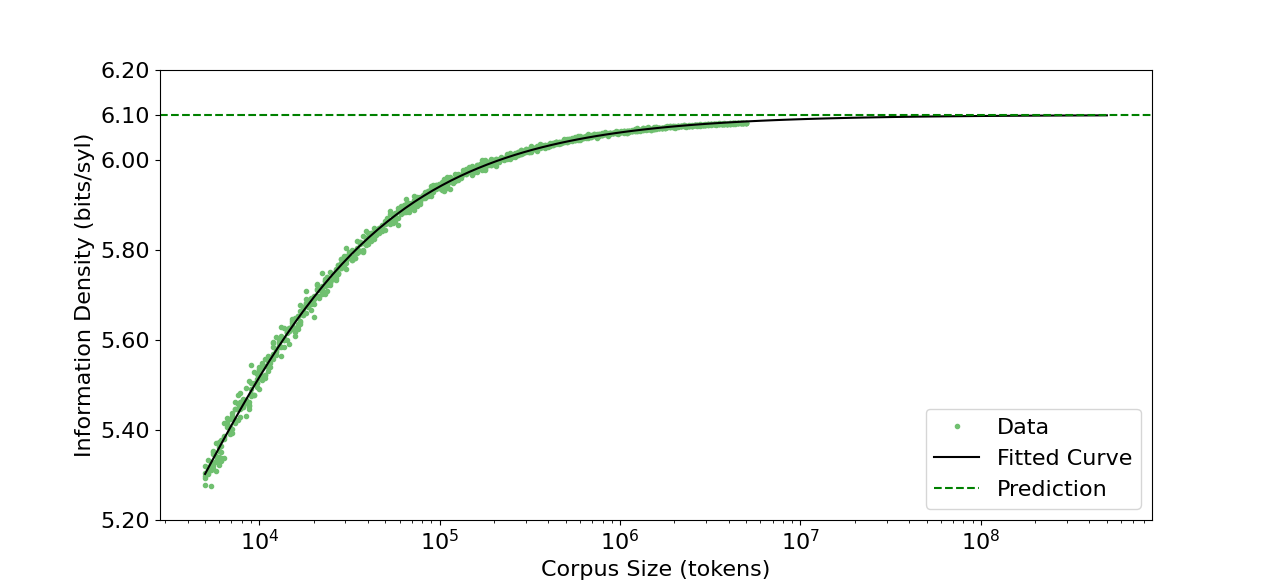
\includegraphics[width=\linewidth]{extrapolation_single}
\end{figure}

\begin{figure}[p]
\centering
\caption{Information density extrapolated from small sub-corpora of English and German (solid line), compared to the result calculated from the entire corpus (dashed line). The difference suggests that expanding the full corpora by another order of magnitude would give us a slightly higher information density.}
\label{fig:exdouble}
\noindent\includegraphics[width=\linewidth]{extrapolation_double}
\end{figure}

Notably, however, the issues with bootstrapping arise from sampling with replacement. By sampling \emph{without} replacement, we can ensure the distribution is preserved. The result is always smaller than the original corpus, but by functionally discarding tokens at random, we can quite reliably create a smaller corpus that maintains the proper distribution. \citet[57]{oh} uses this technique to demonstrate that estimated information density increases sharply with corpus size, then appears to converge (see figure~\ref{fig:exsingle}). We replicated her results for English and German, randomly discarding from the corpora to create smaller sub-corpora and calculating the information density from them. We then attempted to fit a curve to the convergence. In particular, the hyperbola shown in equation~\ref{eq:hyperbola} fit extremely well\footnote{This curve was found empirically to have the best least-squares fit out of several tested, including other hyperbolic curves as well as exponential \(a(1-\exp(-b(x-c)))\) and logarithmic \(a\ln(b(x-c))\).}; it relates the estimated entropy (\(y\)) to the corpus size (\(x\)) with four parameters tuned through least-squares fitting. The results are shown in figure~\ref{fig:exsingle}.

\begin{equation}
\label{eq:hyperbola}
y = a-b(x-c)^{-d}
\end{equation}

To test the extrapolation, we randomly sampled 2 million tokens from the English and German corpora (without replacement), then extrapolated from these smaller sub-corpora (each approximately the size of our original Latin corpus). The results are shown in figure~\ref{fig:exdouble}. For English, extrapolating from the smaller sub-corpus gave an information density of 7.00 bits per syllable, compared to 6.98 calculated from the sub-corpus, 6.98 calculated from the full corpus\footnote{This number differs slightly from \posscite[61]{oh} 7.09 due to differences in the corpus; the exact corpus used by \citeauthor{oh} was not available.}, or 6.99 extrapolated from the full corpus. For German, extrapolating from the smaller sub-corpus gave an information density of 6.11 bits per syllable, compared to 6.08 calculated from the sub-corpus, 6.08 calculated from the full corpus, or 6.10 extrapolated from the full corpus. This implies that 2 million tokens is sufficient for a good estimate on its own, but also gives us confidence in our method of extrapolation.

\subsection{Jackknifing}

Even if the number of tokens is sufficient for a good estimate, using the \emph{entire} corpus of surviving literature raises another issue: how do we know that the corpus is representative of the language? When we discarded tokens from the English and German corpora, we discarded at random, ensuring the result followed the same distribution as the full corpus (and redoing the frequency calculations each time to account for the altered corpus size). But we have no way of knowing whether the works of literature that \emph{didn't} survive had the same distribution as the ones that did\footnote{There is also a question of how accurately written literature represents the spoken language, but this is an issue with any written corpus. Following \citereset\citet{oh} and \citet{coupé}, we ignore it here.}.

In some ways, this is a problem that can't be overcome. Barring a new archaeological find or rediscovered manuscript, the details of the literature that didn't survive are simply unknowable. But using the corpus we \emph{do} have, we can analyze the effect of each individual source on the results, giving a sense of how much our result could be swayed by any particular lost source.

For this purpose, we assume that the differences between authors are more significant than the differences between works. In other words, the loss of Ovid's \emph{Medea} is unlikely to make a significant impact on our calculations, since many other works by Ovid survive. The loss of the complete works of Cornelius Gallus, on the other hand, could matter a great deal, since he would have offered a completely different authorial voice and style---possibly with a much higher or lower information density than the others.

To estimate the impact of our limited pool of authors, we propose a new technique we term \emph{author jackknifing}, named after jackknife resampling in statistics \citep{efron}. In this technique, we calculate the information density of the entire corpus, with one particular author removed---for example, we would calculate the information density of the entire corpus minus the works of Ovid, or the entire corpus minus the works of Livy. The distribution of these values, then, gives a sense of the impact an individual author could have, and we can take the standard deviation of this distribution as an approximation of our standard error. If this uncertainty is low, that suggests that a single author's style is unlikely to have a large impact on the results, and we can be more confident in our estimate.

\section{Results}
\label{sec:res}

The corpus we used is the PHI Latin Corpus, published by the \citet{phi}. It contains ``essentially all Latin literary texts'' from before 200 CE, plus a few later works that are deemed important and distinctly Classical in style\footnote{For example, the corpus includes the commentaries of Servius Honoratus, from the fourth century CE.}. Pretty much any text that's recognizably Classical Latin and part of a published work is included, regardless of length or genre. In particular, we used version 5.3 as distributed on CD, in conjunction with CLTK's index \citep{cltk}, as it made it easier to access full texts than the newer web interface. This version of the corpus includes 329,228 types and 7,240,273 tokens\footnote{These numbers differ from the ones in table~\ref{tab:corpus} because the values here include Justinian and table~\ref{tab:corpus} does not.}, from 362 authors.

However, most of these 362 authors have relatively little contribution---for example, Cornelius Dolabella's only surviving text is the two words \emph{mortem ferre} `to bring death'\footnote{Quoted in Quintilian \citep[VIII.2.4]{quintilian}. A fair number of authors are primarily (or only) known to us through ancient quotations, raising questions about their authenticity or their usefulness for corpus analysis; discussion of some of these problems, and the general practices of quotation in this era, can be found in \citet{vandenhoek}. We follow the decisions of the \citeauthor{phi} in this area, separating out quoted authors wherever the compilers of the corpus deemed it useful to do so.}. Including these would make author jackknifing somewhat useless, since it's clear that two words from an unknown author can't significantly impact the entropy of a seven-million-word corpus. So, for the purposes of jackknifing specifically, we included only authors who contributed more than 100,000 tokens, as shown in table~\ref{tab:corpus}.

\begin{table}[h]
\centering
\caption{The composition of the corpus.}
\label{tab:corpus}
\begin{tabular}{|c|c|c|c|c|}
\hline
\textbf{Author} & \textbf{Genre} & \textbf{Century} & \textbf{Types} & \textbf{Tokens} \\\hline
\textbf{Total} & & & 321,447 & 6,387,500 \\\hline\hline
Cicero & Everything & 1st BCE & 85,020 & 1,165,502 \\\hline
\rowcolor{lightgray} \emph{Justinian} & \emph{Law} & \emph{6th CE} & \emph{40,599} & \emph{852,973} \\\hline
Livy & History & 1st BCE & 55,308 & 520,674 \\\hline
Pliny & Science & 1st CE & 68,237 & 392,178 \\\hline
Servius & Grammar & 4th CE & 52,524 & 373,819 \\\hline
Seneca & Philosophy & 1st CE & 50,723 & 362,937 \\\hline
Quintilian & Rhetoric & 1st CE & 40,092 & 321,209 \\\hline
Ovid & Poetry & 1st BCE & 36,787 & 222,745 \\\hline
Plautus & Comedy & 3rd BCE & 27,352 & 166,390 \\\hline
Tacitus & History & 1st CE & 33,744 & 161,368 \\\hline
Gellius & Notes & 2nd CE & 24,636 & 118,021 \\\hline
Columella & Agriculture & 1st CE & 26,019 & 115,811 \\\hline
``S. H. A.''\tablefootnote{\emph{Scr\=\i{}ptor\=es Historiae Augustae}, literally the ``authors of the Augustan History''. The actual identity of the author, or authors, is unknown.} & Biographies & 4th CE? & 23,892 & 107,893 \\\hline
Apuleius & Novel & 2nd CE & 30,735 & 103,901 \\\hline
Celsus & Religion & 2nd CE & 15,736 & 102,035 \\\hline
Others & & & 189,907 & 2,153,017 \\\hline
\end{tabular}
\end{table}

Using this corpus for analysis, and these fifteen authors for jackknifing, two outliers immediately became apparent.

The first involves Justinian. The \emph{Digesta} of Justinian is one of the later (post-200-CE) works included in the CLTK corpus: a fifty-volume compilation of legal precedents and decisions. Since many of these precedents are from the Classical period, it makes some sense to include them in the corpus. However, they are also extremely formulaic and repetitive (note the very low type/token ratio in table~\ref{tab:corpus})---to the point that they significantly lower the overall information density of the corpus, as shown in figure~\ref{fig:digesta}. Since the \emph{Digesta} was compiled much later than the other works in the corpora, we feel comfortable excluding it as an outlier.

\begin{figure}[h]
\centering
\caption{Estimated information density with and without the \emph{Digesta}.}
\label{fig:digesta}
\noindent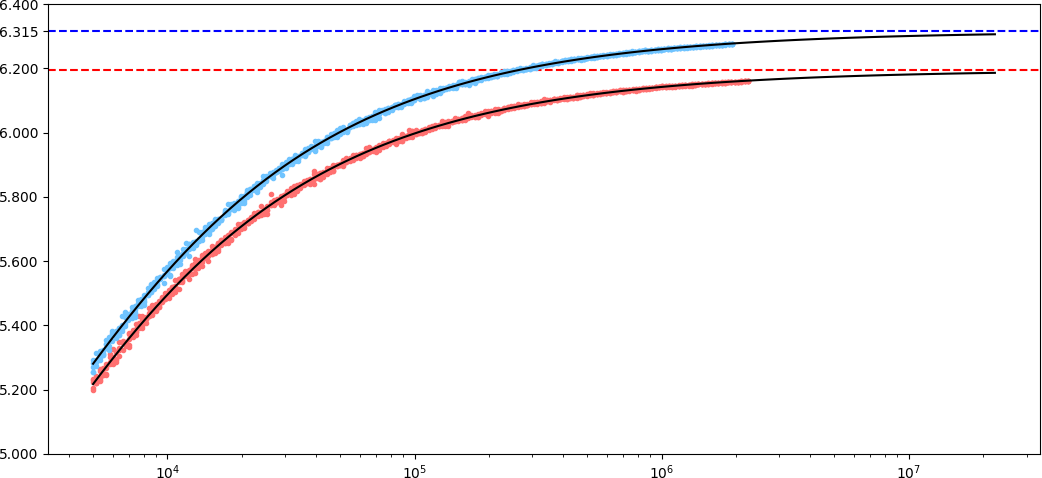
\includegraphics[width=\linewidth]{digesta}
\end{figure}

The second involves Cicero. He was an absurdly prolific writer, and due to the praise of early Christian church fathers, his works were preserved better than most others'---it's estimated that over 75\% of the surviving writings from his lifetime are his \citep{harrison}. Even looking at other time periods, his works make up over 18\% of our corpus. As such, he has a much greater impact on our information density estimate than most other authors, through sheer volume (as can be seen in figure~\ref{fig:jackknifing}).

Arguments could be made to exclude his works from the corpus as an outlier, due to this impact, and also what some have called his ``extremely poor vocabulary''\footnote{This is not to suggest that he didn't know many words, but rather that he deliberately strove for consistency and clarity in his vocabulary, discarding many synonyms and alternate constructions as a result. In his works on oratory, he describes this as a key component of good speech.} \citep[136]{albrecht}. Arguments could also be made to include his works in the total corpus but exclude them from the jackknifing, since some consider Cicero's works definitional to the ``Classical'' style, rather than being just another author \citep[136]{albrecht}. In the end, we decided to include his works both in the corpus \emph{and} in the jackknifing. Even if his vocabulary was deliberately limited, his works are still an important example of Latin written in the Classical period, and from a descriptive standpoint we believe his authorial style should factor into our uncertainty the same as any other author's.

Using this corpus (with Justinian excluded but Cicero included), the results of the extrapolation can be seen in figure~\ref{fig:results}. The information density calculated from the entire corpus is 6.204 bits per syllable, extrapolated to 6.216 bits per syllable.

The results of author jackknifing are shown in figure~\ref{fig:jackknifing}. The mean of the extrapolated entropy of the fourteen resampled corpora is 6.220 bits per syllable, with a standard deviation of 0.0198. This standard deviation approximates how much any particular lost author could impact our results, and we take it as a measure of the uncertainty in our estimate.

\begin{figure}[p]
\centering
\caption{Estimated information density from the entire corpus.}
\label{fig:results}
\noindent\includegraphics[width=\linewidth]{latin}
\end{figure}

\begin{figure}[p]
\centering
\caption{Results of author jackknifing. The visible outlier (in purple) is the corpus without Cicero.}
\label{fig:jackknifing}
\noindent\includegraphics[width=\linewidth]{jackknifing}
\end{figure}

According to \citet{coupé}, the mean information rate across languages is 39.15 bits per second, with a standard deviation of 5.10. From this, we calculate a reconstructed speech rate:

\begin{align}
SR &= \frac{IR}{ID} = 6.29\:\textrm{syl/sec} \\
\sigma_{SR} &= \sqrt{\left(\frac{\sigma_{IR}}{ID}\right)^2 + \left(\frac{\sigma_{ID}}{ID}\right)^2} = 0.82
\end{align}

Notably, the uncertainty in our information density value (\(\sigma_{ID}\)) is so small compared to the natural variation in IR (\(\sigma_{IR}\)) that it becomes negligible. The effect of different authorial styles on our information density estimate is completely drowned out by the size of the ``optimal range'' for IR, suggesting that our corpus is diverse enough to be confident in the results.

\section{Discussion}
\label{sec:disc}

Compared to \posscite{coupé} empirical data, these results---6.29 syllables per second with a standard deviation of 0.82---seem quite reasonable. The rate is fairly similar to that of English, with some other languages being much faster and others much slower. The uncertainty is significantly smaller than many of the differences between languages, showing that our results are precise enough to be meaningful. And the uncertainty is also fairly similar to the variations reported in \citeauthor{coupé}'s experiment.

Figure~\ref{fig:violin1} compares our reconstructed speech rate for Classical Latin against the data gathered by \citet{coupé} for Vietnamese, English, and Japanese. Tickmarks indicate the mean and one standard deviation above and below; for living languages, the ``violin'' of the plot shows the distribution of measurements of actual speech rate, while for Latin, it's approximated by a normal distribution with our calculated mean and standard deviation.

\begin{figure}[p]
\centering
\caption{Our reconstructed speech rate for Classical Latin, compared to measured speech rates of living languages: Vietnamese, English, and Japanese.}
\label{fig:violin1}
\noindent\includegraphics[width=\linewidth]{violin_global}
\end{figure}

\subsection{Comparison}

Now that we know our estimated speech rate is plausible for a language in general, a more interesting question arises: how does it compare to its descendants, the modern Romance languages? Figure~\ref{fig:violin2} compares our reconstructed values for Latin against the measured values for the four Romance languages included in \posscite{coupé} study: Catalan, French, Italian, and Spanish.

Notably, Latin seems to be spoken significantly slower than all the Romance languages tested, often by at least one standard deviation. Spanish, the fastest of them, is more than an entire syllable per second faster.

\begin{figure}[p]
\centering
\caption{The speech rate of Classical Latin compared to modern Romance languages: Catalan, French, Italian, and Spanish.}
\label{fig:violin2}
\noindent\includegraphics[width=\linewidth]{violin_romance}
\end{figure}

The next question is, are there phonological reasons for this? In other words, are there significant phonological differences between Classical Latin and its modern descendants that would explain this significant difference in speech rate? In table~\ref{tab:phono} we reproduce some phonological data from \citet{oh} for comparison\footnote{An estimate of syllable inventory size based on corpus measurements is also reported by \citet{oh}, but not included here. Her method of estimation involves looking at the most frequent lemmata in the corpus, and our Latin corpus has not been lemmatized.}. ``C'', ``V'', and ``T'' indicate the size of the inventory of consonants, vowels, and tone/stress features; ``Complexity'' and ``Index'' are measures of syllable complexity proposed by \citet{wals} and \citet{lapsyd} respectively (the ``index'' being roughly equivalent to the maximum number of segments in a single syllable); and ``SE'' and ``ID'' are the Shannon entropy and information density reported by \citet{oh}, both in bits per syllable.

\begin{table}[h]
\centering
\caption{Phonological statistics for Classical Latin compared to modern Romance languages: number of consonants, vowels, and tone/stress features; complexity and complexity index; Shannon entropy and information density. Romance data from \cite[44-45]{oh}.}
\label{tab:phono}

\vspace{2ex}

\begin{tabular}{|c|c|c|c|c|c|c|c|}
\hline
\textbf{Language} & \textbf{C} & \textbf{V} & \textbf{T} & \textbf{Complexity} & \textbf{Index} & \textbf{SE} & \textbf{ID} \\\hline
Latin & 21 & 17 & 0 & Complex & 7 & 8.71 & 6.22 \\\hline
Catalan & 25 & 8 & 2 & Moderate & 4 & 8.10 & 5.49 \\\hline
French & 22 & 15 & 0 & Complex & 7 & 8.39 & 6.68 \\\hline
Italian & 27 & 7 & 1 & Complex & 6 & 8.32 & 5.29 \\\hline
Spanish & 27 & 5 & 1 & Moderate & 5 & 8.32 & 5.43 \\\hline
\end{tabular}
\end{table}

Notably, the Shannon entropy (SE) of Classical Latin---that is, the syllable entropy without context, as formulated in equation~\ref{eqn:shannon}---is much closer to that of modern Romance languages than the information density (ID). We attribute this mainly to the presence of stress. Phonemic stress, as found in many Romance languages, increases the number of possible syllables immensely (since, for example, stressed \emph{\'a} and unstressed \emph{a} become phonologically distinct syllables). This increase in the syllable inventory then greatly increases the Shannon entropy. But the information density incorporates context as well, and in context, stress matters much less---in stress-accent languages, there tends to be one and only one ictus per word, not an independent binary ``stressed/unstressed'' property for each syllable. Latin lacks phonemic stress but has phonemic vowel length, which is a property of each individual vowel rather than the word: \emph{pila} `ball', \emph{p\=\i{}la} `mortar', \emph{pil\=a} `with a ball', \emph{p\=\i{}l\=a} `with a mortar'. So while the effects of stress and vowel length on the Shannon entropy are similar, their effects on the information density are very different.

The ``Complexity'' and ``Index'' values, while fairly similar here, can also obscure significant differences in syllable structure. Latin generally allows up to three consonants in a coda: \emph{urbs} \ipa{urps} `city', \emph{calx} \ipa{kalks} `chalk'. Italian, on the other hand, does not allow any clusters in codas \citep{hall}. The reason for the similar ``Index'' and ``Complexity'' values is the analysis of diphthongs---the \ipa{a\textsubarch{e}} in Latin \emph{saepe} `often' is taken as a single segment, while the \ipa{a\textsubarch{i}} in Italian \emph{assai} `very' is taken as two segments, for phonological reasons. And the number of possible diphthongs is much smaller than the number of possible consonant clusters.

\subsection{Historical Phonology}

Leaving aside \posscite{lapsyd} index, we suggest a broader look at the history of the Romance languages, and what sorts of common phonological changes these languages shared.

\begin{figure}[h]
\centering
\caption{The vowel inventories of Classical Latin (left) and early Romance (right).}
\label{fig:vowels}
\noindent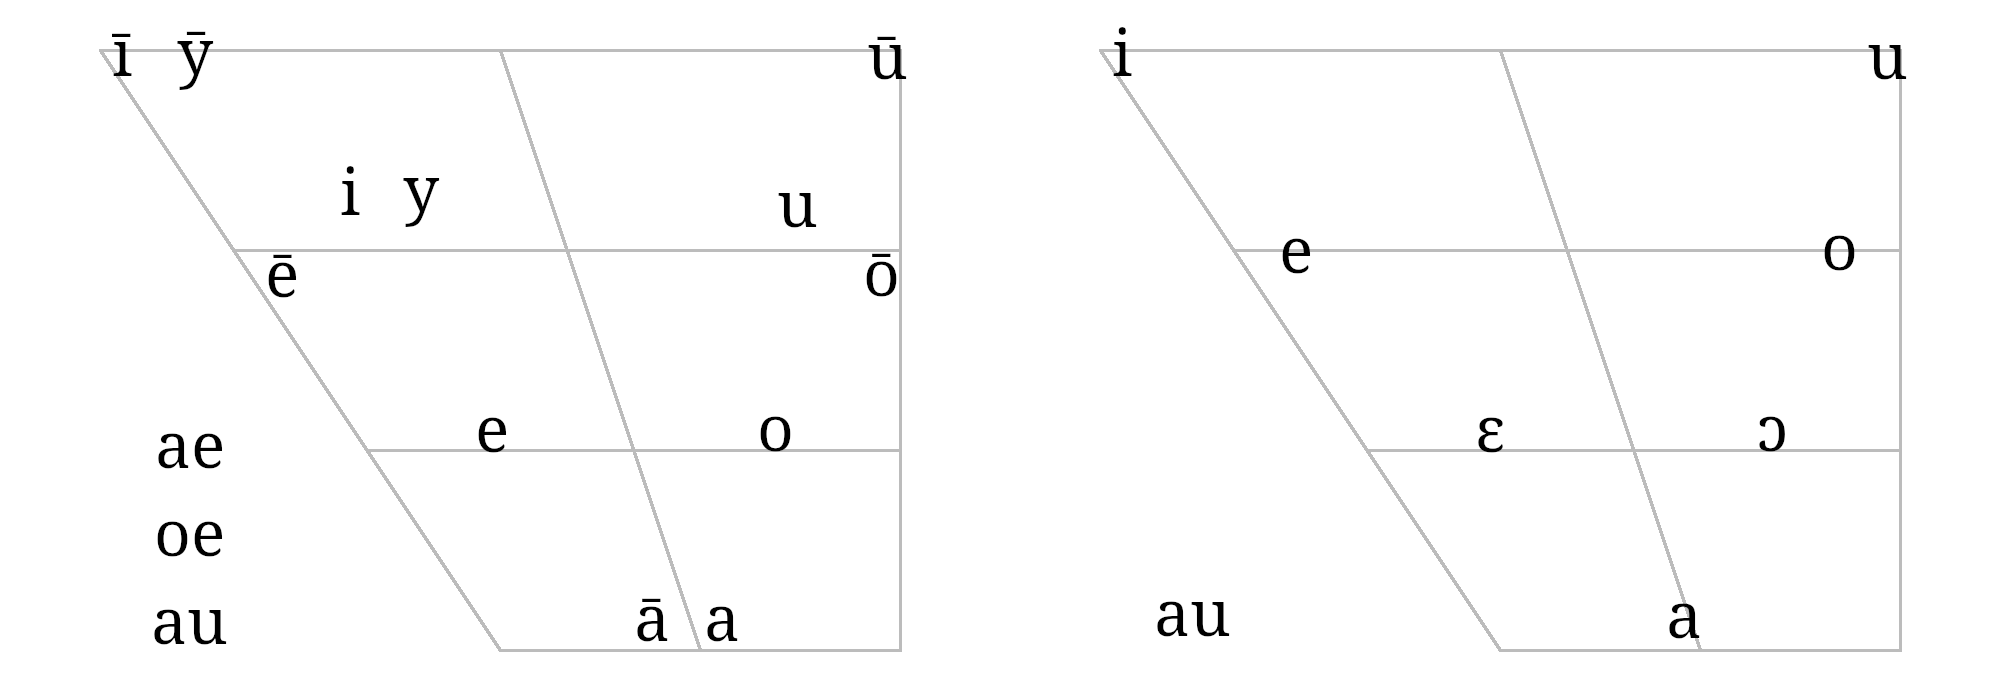
\includegraphics[width=\linewidth]{vowelchange}
\end{figure}

\textbf{Vowel changes}: Classical Latin had twelve phonemic monophthongs, \ipa{i y e a o u} with a binary length distinction, and at least\footnote{Some analyses, such as \citet{allen}, consider other diphthongs phonemic as well, but others, such as \citet{alkire} and \citet{boyd}, include only these three. In this paper, we follow \citeauthor{allen} for most matters of Classical phonology and phonetics (including table~\ref{tab:phono}), but \citet{alkire} specifically in discussions of historical development (including figure~\ref{fig:vowels}).} three phonemic diphthongs, \ipa{a\textsubarch{e} o\textsubarch{e} a\textsubarch{u}}. Early in Proto-Romance, the length distinction became a quality distinction, and a series of mergers resulted in seven phonemic monophthongs \ipa{i e E a O o u} and one diphthong \ipa{a\textsubarch{u}}, as shown in figure~\ref{fig:vowels}. \citet{alkire} refer to this as the ``Great Merger'', and its effects can be seen in almost all Romance languages\footnote{The famous exception is Sardinian.}; most underwent further mergers, especially in unstressed position \citep{alkire,boyd}. The main result of this was to cut the number of possible syllables nearly in half.

\textbf{Cluster breaking}: While Classical Latin allowed \ipa{s} before stops in onsets, Western Romance varieties historically did not.

\begin{exe}
\ex \emph{strictus} `tight' \yields{} Spanish \emph{estrecho}
\ex \emph{sponsa} `fiancée' \yields{} Old French \emph{espose} \yields{} French \emph{épouse}
\ex \emph{scriptus} `written' \yields{} Catalan \emph{escrit}
\end{exe}

This prohibition eventually weakened in some languages (such as Modern French), and the epenthetic vowels mostly disappeared in Italian---\emph{stretto}, \emph{sposa}, \emph{scritto}---though relics like \emph{iscritto} survive in fossilized phrases\footnote{Some older speakers have also been reported to preserve the epenthetic vowel when the word follows a consonant: \emph{alla Svizzera} but \emph{in Isvizzera}.} \citep{alkire}. But the primary effect was to break up inherited consonant clusters, increasing the number of syllables per word and decreasing the number of possible onsets.

\textbf{Coda loss}: Classical Latin allowed a wide variety of coda consonants, including stops, nasals, and fricatives. Many of these disappeared in the development of Romance, especially word-finally:

\begin{exe}
\ex \emph{hab\=etis} `you all have' \yields{} Italian \emph{avete}
\ex \emph{ferrum} `iron' \yields{} Catalan \emph{ferro}
\ex \emph{am\=abat} `she was loving' \yields{} Spanish \emph{amaba}
\end{exe}

Certain codas were already being lost in the Classical period---poetry and inscriptions indicate that coda \ipa{m}, while phonologically present, was no longer realized as a separate segment\footnote{In other words, it was probably realized as nasalization of the preceding vowel instead of as a consonant \ipab{m}.}---and some Romance branches took this process farther than others. Latin \emph{serv\=os} `slaves', for instance, became Spanish \emph{siervos} but Italian \emph{servi} (via an intermediate *\emph{servoj}). This contributed, again, to a decrease in the inventory of possible syllables.

\textbf{Consonant loss and gain}: Some Classical consonants merged or disappeared without a trace in Romance, while some others arose out of previously non-phonemic contrasts:

\begin{exe}
\ex \emph{hortus} `garden' \yields{} Old French \emph{ort}
\ex \emph{chorus} `chorus' \yields{} Spanish \emph{coro}
\ex \emph{f\=ageus} \ipa{fa:geus} `beech' \yields{} Italian \emph{faggio} \ipa{faddZo}
\end{exe}

The result is a similar number of consonants in Classical Latin and its descendants, as reported in table~\ref{tab:phono}. While the inventory of consonants varies significantly, its size is similar between Latin and the Romance languages surveyed.

\textbf{Syncope}: Many unstressed medial vowels were deleted very early in the history of Romance. This change happened early enough to appear in inscriptions, and in a few cases the effects are even visible during the Classical period:

\begin{exe}
\ex \emph{calida} `hot' \yields{} Latin \emph{calda}\footnote{The emperor Augustus is quoted by Quintilian \citep[I.6.19]{quintilian} as calling the longer form ``superfluous'' and telling his grandson to avoid it.} \yields{} Italian \emph{calda}
\ex \emph{viridis} `green' \yields{} Spanish \emph{verde}
\ex \emph{altera} `other' \yields{} Old French \emph{altre} \yields{} French \emph{autre}
\end{exe}

This created more consonant clusters---but, crucially, did not significantly increase the inventory of syllables, or allow syllables to appear in more contexts. All of these clusters and syllables existed in the language before the syncope process took place.

\textbf{French vowel changes}: French is one of the less conservative Romance languages, phonologically, and in particular it has a significantly larger vowel inventory than Italian, Spanish, or Catalan. These vowels stem from a variety of dramatic changes from early Gallo-Romance, often conditioned by surrounding consonants which later disappeared \citep{pope,boyd}:

\begin{exe}
\ex \emph{for\textbf{es}tem} `forest' \yields{} \emph{for\textbf{\^e}t} \ipa{fOKE}
\ex \emph{d\textbf{en}tem} `tooth' \yields{} \emph{d\textbf{en}t} \ipa{d\~A}
\ex \emph{p\textbf{e}dem} `foot' \yields{} \emph{p\textbf{ie}d} \ipa{pje}
\end{exe}

The result is a much larger vowel inventory than the other Romance languages surveyed. This increased the French syllable inventory significantly; we hypothesize that this contributed to the language's relatively high information density, as shown in table~\ref{tab:phono}.

In summary, we believe there are several historical reasons to expect modern Romance languages to have smaller syllable inventories than Latin. This reduces the informational load on each syllable and the difficulty of recognizing syllables, allowing the language to be spoken faster. While syllable frequency likely plays an important role as well, it is notable that the Romance language closest in speech rate to Latin, out of those surveyed, is French---which has a significantly larger vowel inventory than the rest.

\section{Conclusion}
\label{sec:concl}

In this study, we used a variety of tools to analyze the information density of Classical Latin from a written corpus. Applying our new methods of extrapolation and author jackknifing, we came up with an information density of 6.216 bits per syllable, with a standard error of 0.198. Applying these values to \posscite{coupé} information rate distribution, we predict a mean speech rate of 6.29 syllables per second, with a standard deviation of 0.82---significantly slower than the modern Romance languages tested by \citeauthor{coupé}. We believe these results make sense, based on a broad overview of historical developments in Romance.

We believe these methods of extrapolation can be applied to other corpora. While we demonstrated that 2 million tokens is enough, more research is required to determine how small a corpus is sufficient for a good extrapolation. Future work might put a lower bound on this, and potentially apply it to other languages with less written data available.

We've also looked at a handful of prominent historical sound changes to explain our results, but in a language family as well-understood as Romance, we've barely scratched the surface of the potential. With a more detailed investigation of one particular language's historical phonology, it might be possible to trace the evolution of the language's speech rate over time and quantify the effect of particular phonological changes.

Finally, the Latin corpus may offer an opportunity to expand on \citet{oh} and \posscite{coupé} work. They relied solely on within-word context due to the limitations of the available corpora---for many languages, it can be difficult to find good corpora that are both phonemically annotated and include broader context. But Latin orthography is quite close to phonemic, as discussed in section \ref{subsec:repr}, and between-word sandhi effects in Latin have long been studied for the same reason as syllabification: they have a significant impact on metered poetry. This could make it a good test subject for the effects of inter-word context.

The recent advances in the study of linguistic information are exciting, and we believe they have significant potential. Reconstructing phonetic properties of long-dead languages may be only the beginning.

\section*{Supplemental Materials}

The source code used for this analysis can be found at \url{https://github.com/dstelzer/latin-speech-rate}.

\section*{Acknowledgements}

I would like to thank Ryan Shosted for advice and guidance on every part of this project, Yoon Mi Oh for pointers on the entropy calculations, and Tim Stelzer and Ada Stelzer for mathematical assistance.

I would also like to thank the organizers and reviewers of the LSRL 51 conference where this work was first presented; Keith Tse, Benjamin Tucker, William Balla-Johnson, José Ignacio Hualde, and Ed Rubin for their questions and comments at that conference; and three anonymous reviewers for their feedback and insights.

%\nocite{*}
\label{sec:refs}
\setlength\bibitemsep{0.5\baselineskip}
\printbibliography

\end{document}
